% !TEX root =  bopp.tex

%We evaluate our BOPP framework in two case studies that represent different use cases for Bayesian optimization. In both problem settings Bayesian optimization serves to minimize the number of evaluations needed for a computationally expensive operation. The first problem is hyperparameter optimization for probabilistic programs. Here the expensive step is marginalization over the non-optimized random variables in a program, which is performed using one of the generic inference methods provided by Anglican's inference back end. In the second case study we consider programs in which an expensive forward simulation is used to perform approximate Bayesian computation. Here the use of probabilistic programming allows determination of parameters that are marginally optimal with respect to some distribution of simulation inputs.

\begin{figure*}[t]
	%	\includegraphics[width=1.35in,trim={0 0 0 0},clip]{figures/simple-bimodal/simple-bimodal-160229-03-5.png}
	%	\includegraphics[width=1.35in]{figures/simple-bimodal/simple-bimodal-160229-03-10.png}
	%	\includegraphics[width=1.35in]{figures/simple-bimodal/simple-bimodal-160229-03-20.png}
	%	\includegraphics[width=1.35in]{figures/simple-bimodal/simple-bimodal-160229-03-50.png}
	%\includegraphics[width=1.65in]{"figures/simple-bimodal/simple-bimodal-160229-03-100"}
	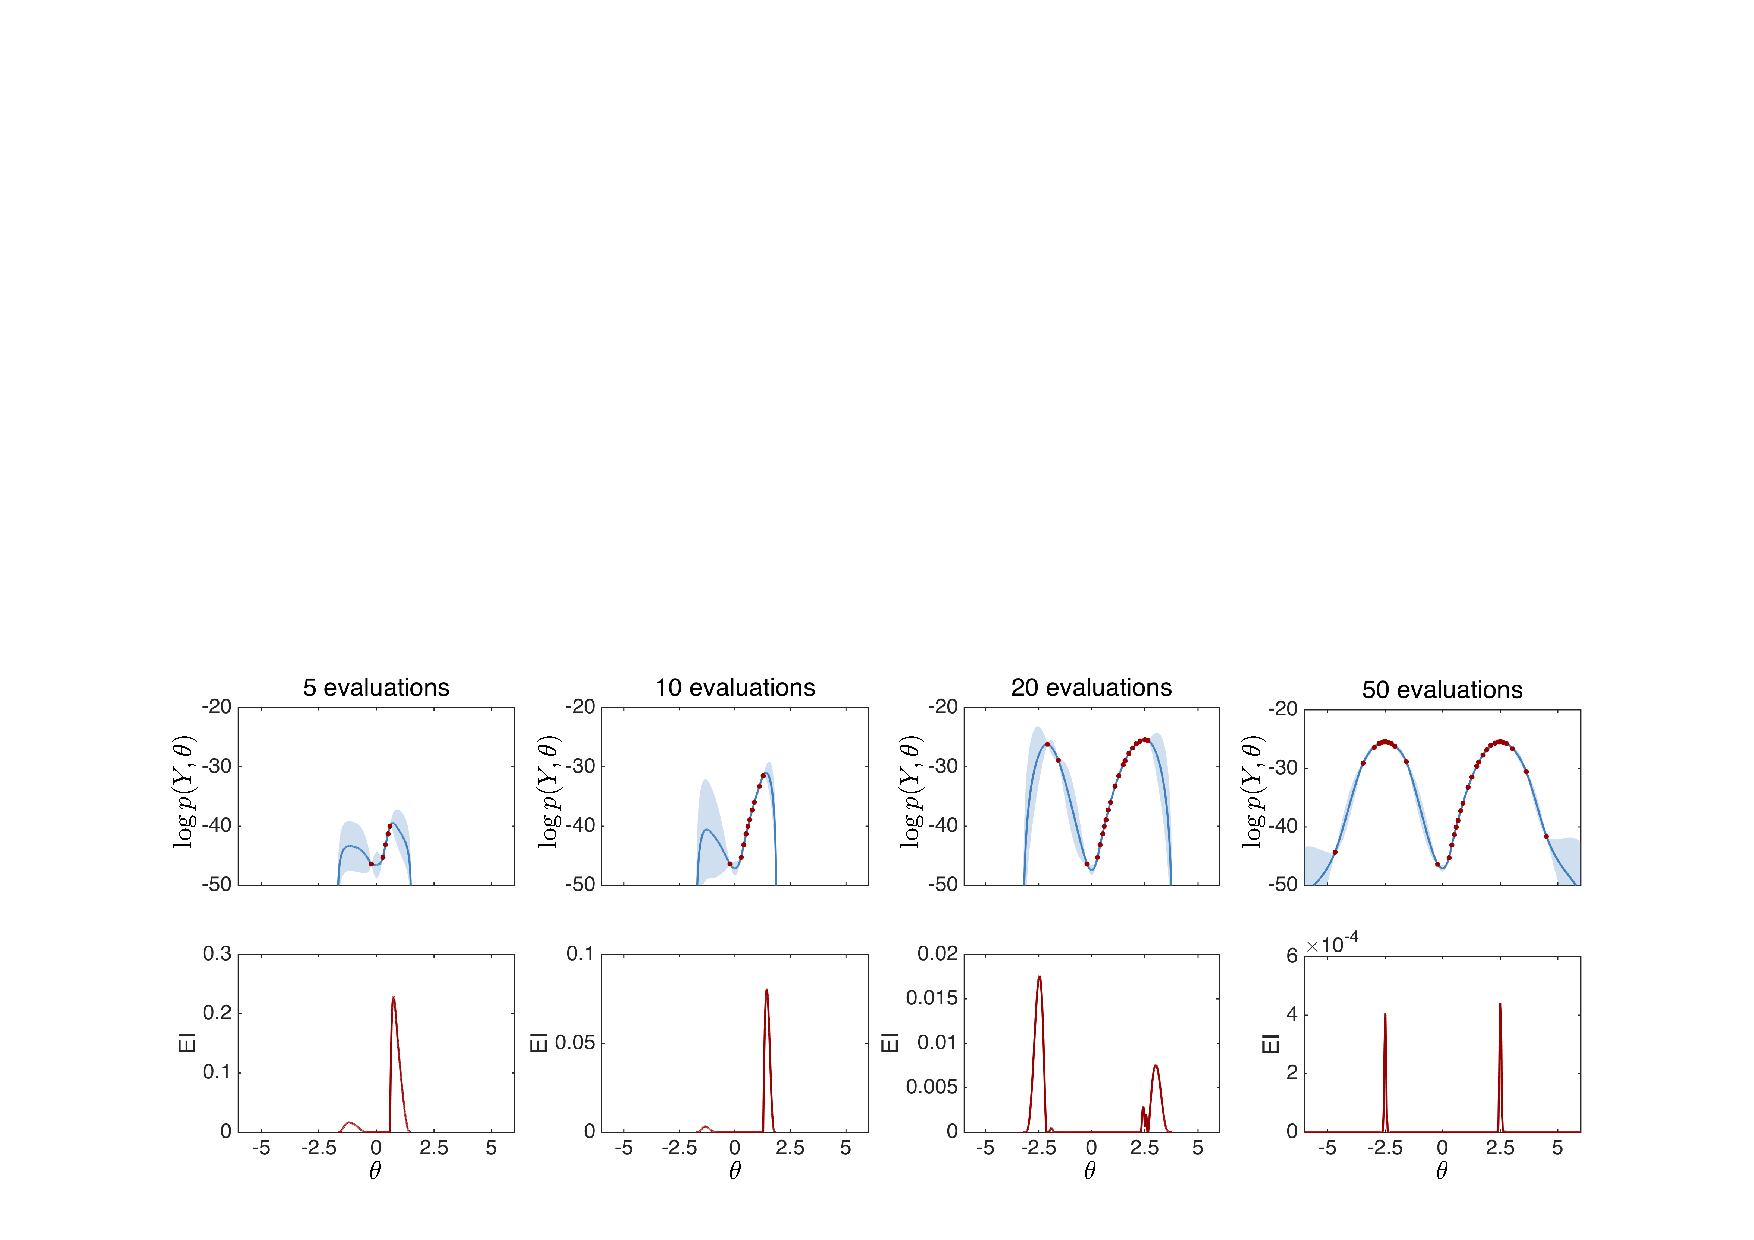
\includegraphics[width=0.99\textwidth]{unbounded_opt}
	\caption{Convergence on an unconstrained bimodal problem with $p \left(\theta\right)={\rm Normal}(0, 0.5)$ and $p \left(Y|\theta\right)={\rm Normal}(5-\left|\theta\right|,0.5)$ giving significant prior misspecification. The top plots show a regressed GP, with the solid line corresponding to the mean and the shading shows $\pm$ 2 standard deviations.  The bottom plots show the corresponding acquisition functions. \label{fig:domainAdpat}}
\end{figure*}

We first demonstrate the ability of BOPP to carry out unbounded optimization using a 1D problem with a significant prior-posterior mismatch as shown in Figure \ref{fig:domainAdpat}.  It shows BOPP adapting to the target and effectively establishing a maxima in the presence of multiple modes.   After 20 evaluations the acquisitions begin to explore the right mode, after 50 both modes have been fully uncovered.

\begin{figure*}[t]
	\centering
	
\includegraphics[width=1\textwidth]{combined_opt_plots}
	%	\includegraphics[width=1.35in]{figures/bayes-opt-comp/branin.pdf}
	%	\includegraphics[width=1.35in]{figures/bayes-opt-comp/hartmann.pdf}
	%	\includegraphics[width=1.35in]{figures/bayes-opt-comp/svm.pdf}
	%	\includegraphics[width=1.35in]{figures/bayes-opt-comp/lda.pdf}
	\caption{Comparison of BOPP  used as an optimizer to prominent BO packages on common benchmark problems.  
		%Branin and Hartmann 6D represent are continuous optimizations, whilst SVM on-grid and LDA on-grid are discrete.  
		The dashed lines shows the final mean error of SMAC (red), Spearmint (green) and TPE (black) as quoted by \cite{eggensperger2013towards}. % which also provides further details on the other packages and the benchmark problems.  
		The dark blue line shows the mean error for BOPP averaged over 100 runs, whilst the median and 25/75\% percentiles are shown in cyan. Results for Spearmint on Branin and SMAC on SVM on-grid are omitted because both BOPP and the respective algorithms averaged zero error to the provided number of significant figures in \cite{eggensperger2013towards}.
		%, meaning it not possible to check where BOPP performed better or worse then the alternative in these two cases.
		\label{fig:bayes-opt}}
\end{figure*}

\subsection{Classic Optimization Benchmarks}

Next we compare BOPP to the prominent BO packages SMAC \cite{hutter2011sequential}, Spearmint \cite{snoek2012practical} and TPE \cite{bergstra2011algorithms} on a number of classical benchmarks as shown in Figure \ref{fig:bayes-opt}.  These results demonstrate that BOPP provides substantial advantages over these systems when used simply as an optimizer on both continuous and discrete optimization problems.  In particular, it offers a large advantage over SMAC and TPE on the continuous problems (Branin and Hartmann), due to using a more powerful surrogate, and over Spearmint on the others due to not needing to make approximations to deal with discrete problems.

\subsection{Marginal Maximum a Posteriori Estimation Problems}

We now demonstrate application of BOPP on a number of MMAP problems.  Comparisons here are more difficult due to the dearth of existing alternatives for PPS.  In particular, simply running inference on the original query does not return estimates for $p\left(Y,\theta\right)$.  We consider the possible alternative of using our conditional code transformation to design a particle marginal Metropolis Hastings (PMMH, \cite{andrieu2010particle}) sampler which operates in a similar fashion to BOPP except that new $\theta$ are chosen using a MH step instead of actively sampling with BO.
%\footnote{To carry out MMAP one could further apply an annealing to the PMMH.  We omit this here as the behaviour of such as system would be indistinguishable from the presented results, due to the small number of iterations and very large variations of $p\left(\theta\right)$ for changes in $\theta$.}
For these MH steps we consider both LMH \citep{wingate2011lightweight} with proposals from the prior and the random-walk MH (RMH) variant introduced in Section \ref{sec:optacqfunc}.

\subsubsection{Hyperparameter Optimization for Gaussian Mixture Model}

% !TEX root =  bopp.tex


\begin{figure}[t]
	\begin{lstlisting}[basicstyle=\footnotesize\ttfamily]
(defopt mvn-mixture [data mu0 kappa psi] [nu alpha]
 (let [[n d] (shape data)
       alpha (sample (uniform-continuous 0.01 100))
       nu (sample (uniform-continuous (- d 1) 100))
       obs-proc0 (mvn-niw mu0 kappa nu psi)]
       (loop [data data
              obs-procs {}
              mix-proc (dirichlet-discrete 
                          (vec (repeat d alpha)))]
	    (let [y (first data)]
	     (if y
	      (let [z (sample (produce comp-proc))
	            obs-proc (get obs-procs z obs-proc0)
	            obs-dist (produce obs-proc)]
	        (observe obs-dist y)
	        (recur (rest data)
	               (assoc obs-procs z (absorb obs-proc y))
	        (absorb mix-proc z)))
	      mix-proc)))))
	\end{lstlisting}
	\caption{
		\label{fig:mvn-code}
		Anglican query for hyperparameter optimization of a Gaussian mixture model, defined in terms of two parameters \lsi{nu} and \lsi{alpha}. A \lsi{mvn-niw} process is used to represent the marginal likelihood of observations under a Gaussian-inverse-Wishart prior, whereas a \lsi{dirichlet-discrete} process models the prior probability of cluster assignments under a Dirichlet-discrete prior. The command \lsi{produce} returns the predictive distribution for the next sample from a process. \lsi{absorb} conditions on the value of the next sample.}
\end{figure}

\begin{figure*}[t]
	%	\includegraphics[width=1.7in]{"../figures/mvn-mixture/opt-nu-alpha-160229-01-10"}
	%	~
	%	\includegraphics[width=1.7in]{"../figures/mvn-mixture/opt-nu-alpha-160229-01-20"}
	%	~
	%	\includegraphics[width=1.7in]{"../figures/mvn-mixture/opt-nu-alpha-160229-01-50"}
	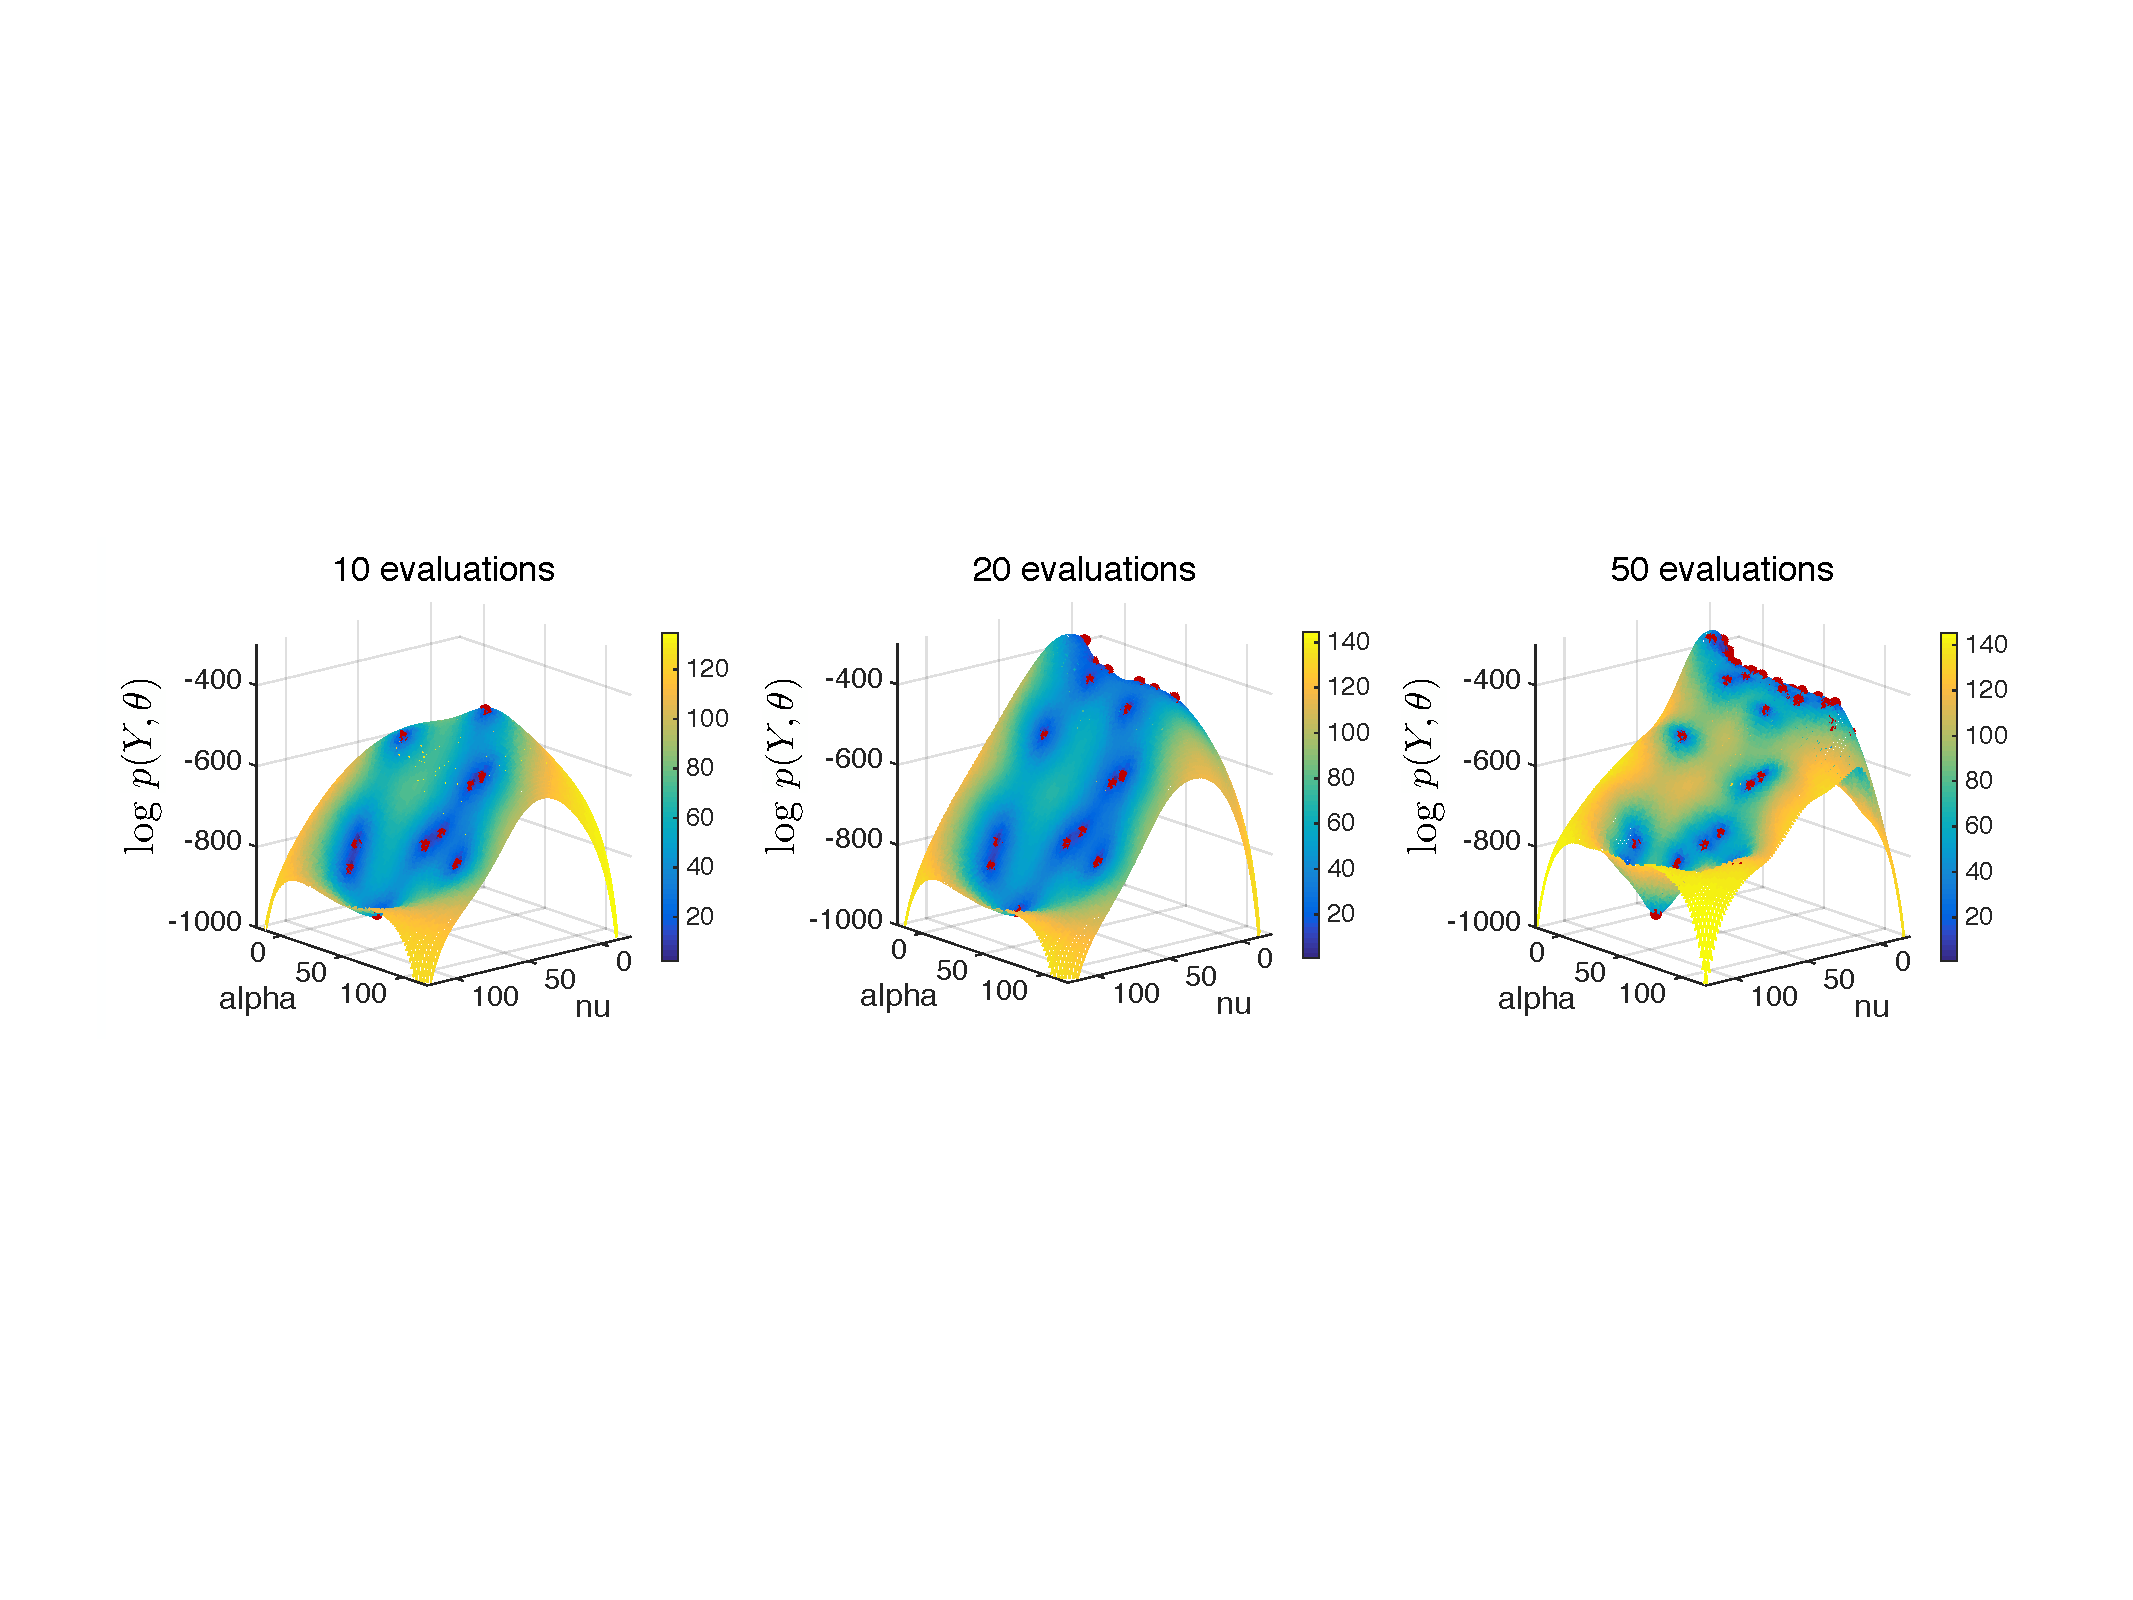
\includegraphics[width=\textwidth]{mvn-mixture/axis_corr_mvn_gps}
	\caption{
		\label{fig:mvn-gp-surface}
		Bayesian optimization of hyperparameters in a Gaussian mixture model evaluated on the Iris dataset. Panels show the GP posterior as a function of number of evaluations, with the surface corresponding to the posterior mean and the color bars the posterior standard deviation. Optimization is performed over the parameter $\alpha$ of a 10-dimensional symmetric Dirichlet distribution and the degrees of freedom $\nu$ of the inverse-Wishart prior. At each evaluation we obtain an estimate of the log marginal $\log p(Y,\theta)$ obtained by performing sequential Monte Carlo inference with 1000 particles.  The apparent maximum after initialization with 10 randomly sampled points lies at $\nu=31$, $\alpha=60$, and $\log p(Y,\theta) = -456.3$ (\emph{left}).  The surface after 10 optimization steps shows a new maximum at $\nu=9.2$, $\alpha=0.8$, and $\log p(Y,\theta) = -364.2$ (\emph{middle}). After 40 steps and 50 total evaluations this optimum is refined to $\nu=16$, $\alpha = 0.2$, and $\log p(Y,\theta) = -352.5$  (\emph{right}).}
\end{figure*}

We start with an illustrative case study of optimizing the hyperparameters in a multivariate Gaussian mixture model. We consider a Bayesian formulation with a symmetric Dirichlet prior on the mixture weights and a Gaussian-inverse-Wishart prior on the likelihood parameters:
\begin{align}
\v{\pi}
&\sim 
{\rm Dir(\alpha, \ldots, \alpha)}
\displaybreak[0]\\
(\v{\mu}_k, \v{\Sigma}_k)
&\sim 
{\rm NIW} (\v{\mu}_0, \kappa, \v{\Psi}, \nu)
&
{\rm for~}
&
k = 1, \ldots , K
\displaybreak[0]\\
z_n 
&\sim 
{\rm Disc(\v{\pi})}
\displaybreak[0]\\
\v{y}_n
&
\sim
{\rm Norm}(\v{\mu}_{z_n}, \v{\Sigma}_{z_n})
&
{\rm for~}
&
n = 1, \ldots , N
\end{align}
% Figure~\ref{fig:mvn-code} shows an optimization query for an Anglican program corresponding to this model. 
Anglican code for this model is shown in Figure 4. Anglican provides stateful objects, which are referred to as random processes, to represent the predictive distributions for the cluster assignments $z$ and the observations $\v{y}^k$ assigned to each cluster
\begin{align}
z_{n+1}
& \sim 
p( \cdot \,|\, z_{1:n}, \alpha),
\\
\v{y}_{m+1}^{k} 
& \sim 
p(\cdot \,|\, \v{y}^k_{1:m}, \v{\mu}_0, \kappa, \v{\Psi}, \nu).
\end{align}
In this collapsed representation marginalization over the model parameters $\v{\pi}$, $\v{\mu}_{k=1:K}$, and $\v{\Sigma}_{k=1:K}$ is performed analytically.
%The only variables that are sampled during program execution are the cluster assignments $z_{1:N}$, which we marginalize over using the general-purpose sequential Monte Carlo (SMC) implementation provided by the inference back end. 
%Like any importance sampling method, SMC provides an unbiased estimate $\hat Z$ of the marginal likelihood $Z = p(\v{y}_{1:N} | \alpha, \v{\mu}, \kappa, \v{\Psi}, \nu)$. 
%Intuitively, the parameter $\nu$, which is known as the degrees of freedom, represents a scale factor for the covariance matrix, which determines the spatial extent of the clusters (larger $\nu$ values imply a smaller covariance and cluster size). 
%The parameter $\alpha$, sometimes known as a concentration parameter, controls the distribution on mixture weights (where $\alpha \gg 1.0$ implies an even distribution and $\alpha \ll 1.0$ implies an uneven distribution).  
Using the Iris dataset, a standard benchmark for mixture models that contains 150 labeled examples with 4 real-valued features, we optimize the marginal with respect to the subset of the parameters $\nu$ and $\alpha$ under uniform priors over a fixed interval.  For this model, BOPP aims to maximize
\begin{align}
\begin{split}
& p(\nu, \alpha | \v{y}_{n=1:N}, \v{\mu}_0, \kappa, \v{\Psi}) \\
&= \iiiint p(\nu, \alpha, z_{n=1:N}, \v{\pi}, \v{\mu}_{k=1:K}, \v{\Sigma}_{k=1:K} | \v{y}_{n=1:N}, \mu_0, \kappa, \v{\Psi}) \mathrm{d}z_{n=1:N}\mathrm{d}\v{\pi}\mathrm{d}\v{\mu}_{k=1:K}\mathrm{d}\v{\Sigma}_{k=1:K}.
\end{split}
\end{align}

Figure~\ref{fig:mvn-gp-surface} shows GP regressions on the evidence after different numbers of the SMC evaluations have been performed on the model.  This demonstrates how the GP surrogate used by BO builds up a model of the target, used to both estimate the expected value of $\log p(Y,\theta)$ for a particular $\theta$ and actively sample the $\theta$ at which to undertake inference.

% n=10
% x1_max: 30.90
% x2_max: 61.55
% y_max: -456.32
% mu_max: -456.33
% sig_max: 0.51

% n=20
% x1_max: 9.20
% x2_max: 0.79
% y_max: -364.21
% mu_max: -364.23
% sig_max: 0.47

% n=50
% x1_max: 16.34
% x2_max: 0.21
% y_max: -352.51
% mu_max: -352.51
% sig_max: 0.53

% n=100
% x1_max: 16.34
% x2_max: 0.21
% y_max: -352.51
% mu_max: -352.50
% sig_max: 0.41

% \begin{figure}
% \begin{lstlisting}[basicstyle=\footnotesize\ttfamily]
% (defopt mvn-mixture 
%  [data mu kappa psi] [:nu :alpha]
%  (let [[n d] (shape data)
%        alpha (sample :alpha
%               (uniform-continuous 0.01 100))
%        nu (sample :nu 
%            (uniform-continuous (- d 1) 100))
%        obs-proc0 (mvn-niw mu kappa nu psi)]
%   (loop [data data
%          obs-procs {}
%          mix-proc (dirichlet-discrete 
%                    (vec (repeat d alpha)))]
%    (let [y (first data)]
%     (if y
%      (let [z (sample (produce comp-proc))
%            obs-proc (get obs-procs 
%                      z obs-proc0)
%            obs-dist (produce obs-proc)]
%       (observe obs-dist y)
%       (recur (rest data)
%              (assoc obs-procs
%                z (absorb obs-proc y))
%              (absorb mix-proc z)))
%      (predict mix-proc))))))
% \end{lstlisting}
% \caption{
% \label{fig:mvn-code}
% Anglican query for hyperparameter optimization of a Gaussian mixture model, defined in terms of two parameters \lsi{:nu} and \lsi{:alpha}. A \lsi{mvn-niw} process is used to represent the marginal likelihood of observations under a Gaussian-inverse-Wishart prior, whereas a \lsi{dirichlet-discrete} process models the prior probability of cluster assignments under a Dirichlet-discrete prior. The command \lsi{produce} returns the predictive distribution for the next sample from a process. \lsi{absorb} conditions on the value of the next sample.}
% \end{figure}





% 


\subsubsection{Extended Kalman Filter for the Pickover Chaotic Attractor}
\label{sec:AppKalman}

% !TEX root =  ../main.tex


\begin{figure*}[t]
	\centering
	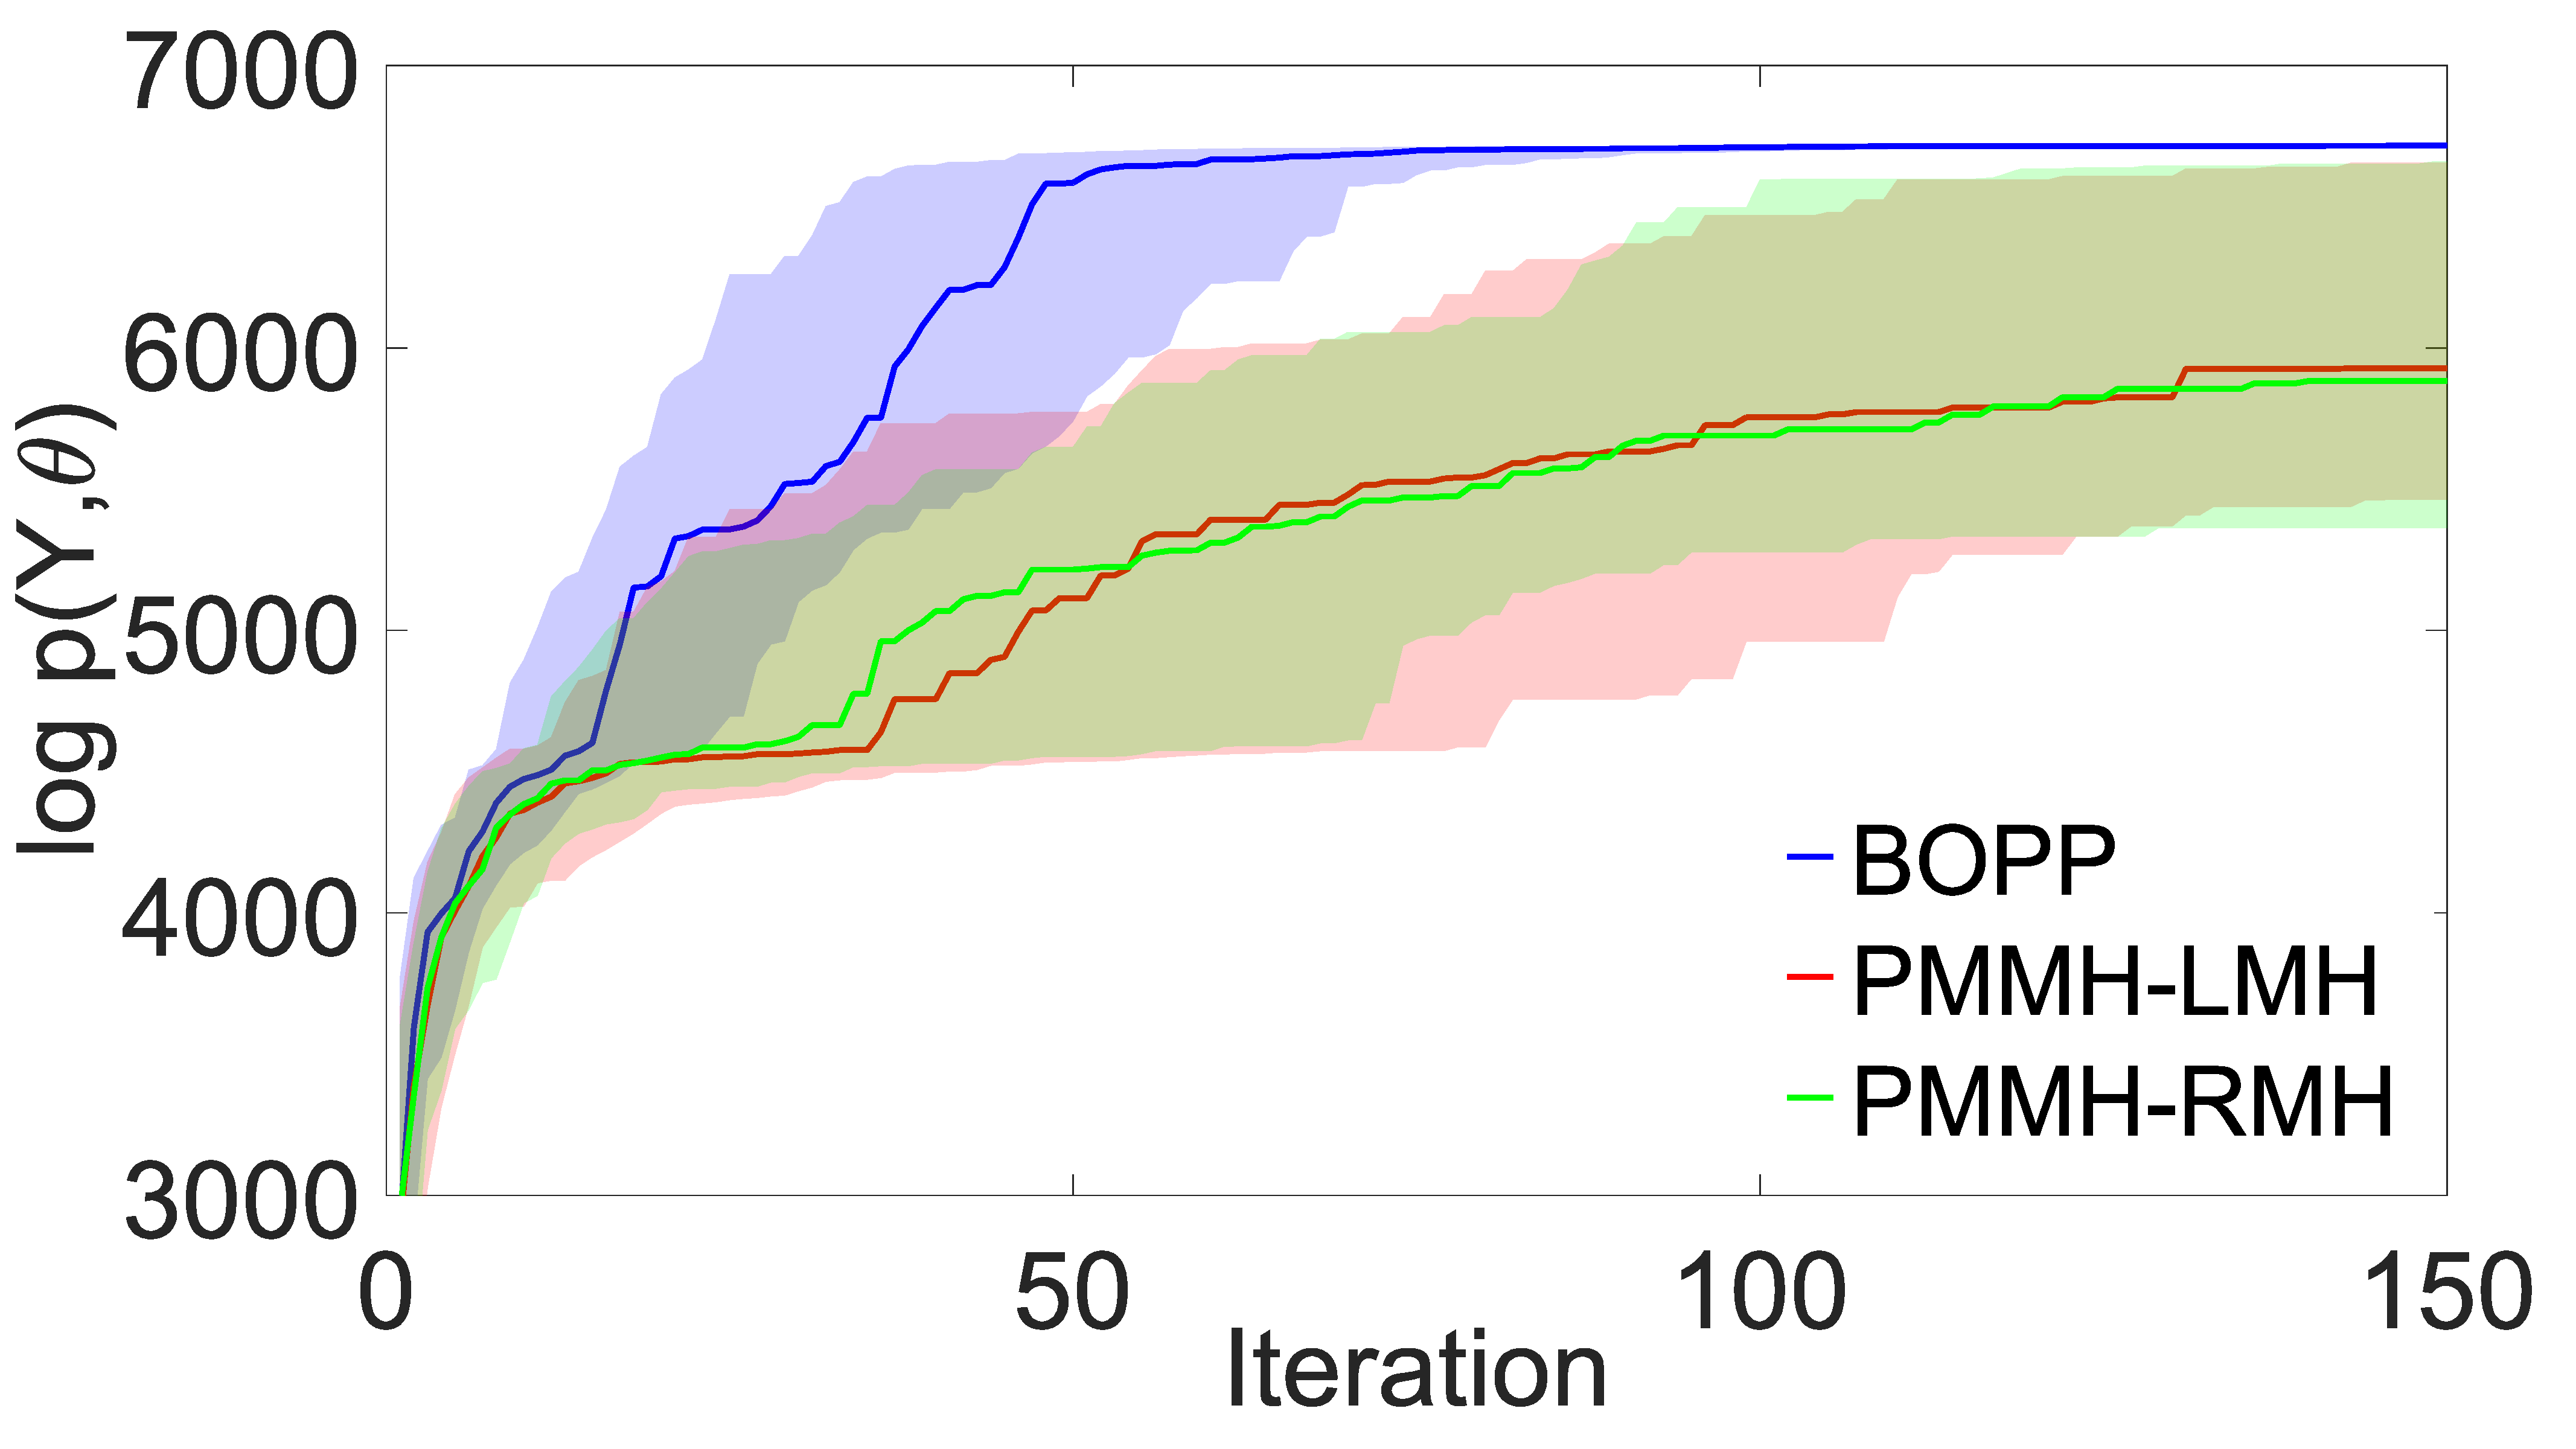
\includegraphics[width=2.72in]{chaos/chaos_ml.pdf}
	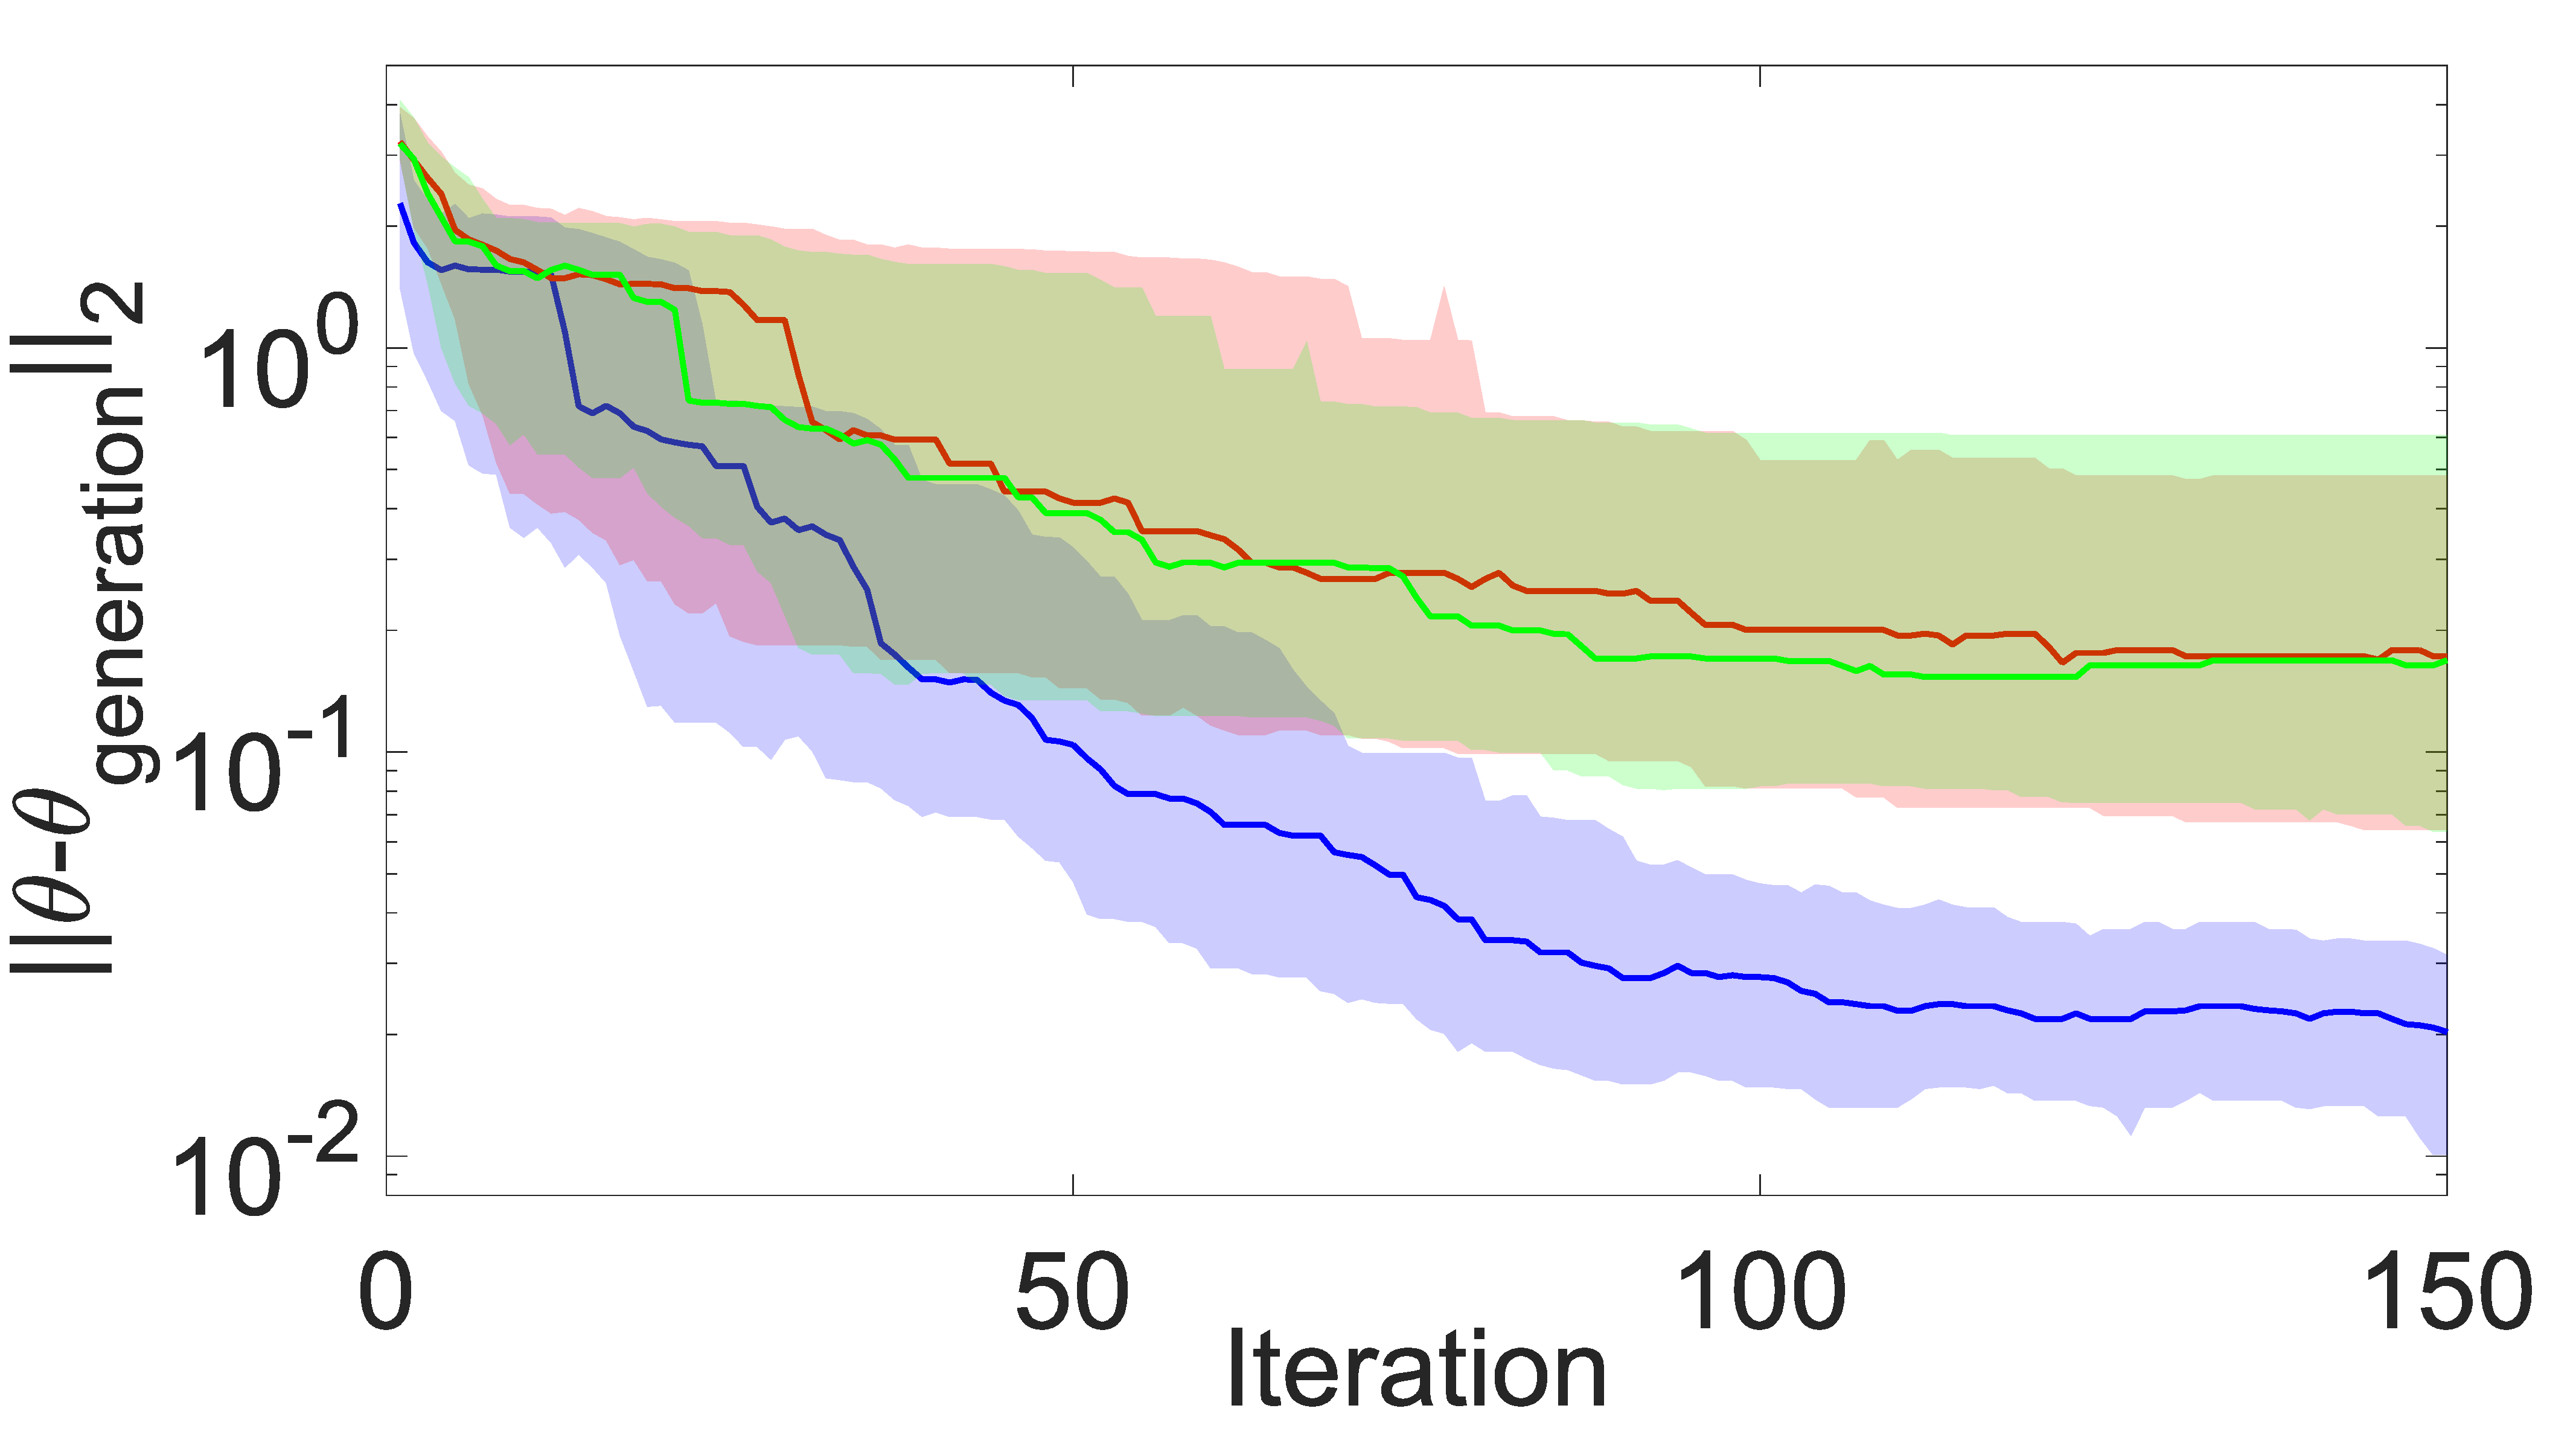
\includegraphics[width=2.72in]{chaos/chaos_distance.pdf}
	\caption{Convergence for transition dynamics parameters of the pickover attractor in terms of the cumulative best $\log p\left(Y,\theta\right)$ (\emph{left}) and distance to the ``true" $\theta$ used in generating the data (\emph{right}). Solid line shows median over 100 runs, whilst the shaded region the 25/75\% quantiles.  \label{fig:chaos}
		\vspace{6pt}}
\end{figure*}

\begin{figure}[t]
	\centering
	\begin{subfigure}[t]{0.24\textwidth}
		\centering
		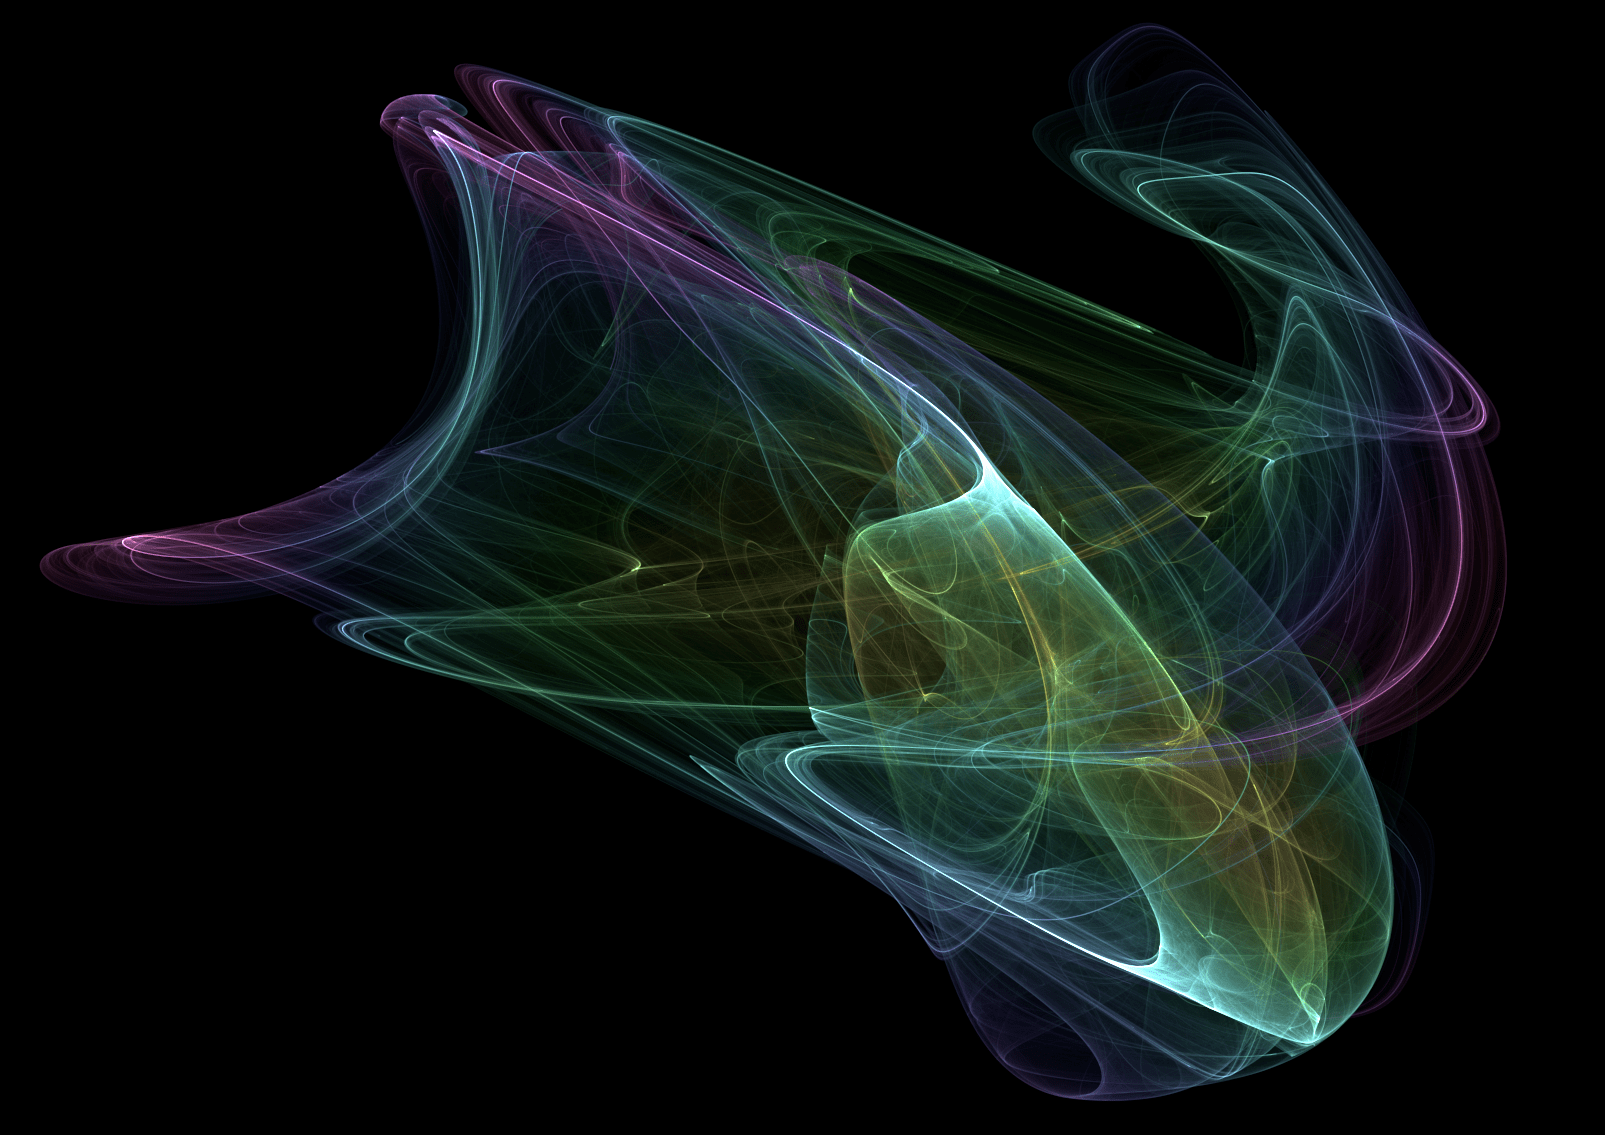
\includegraphics[height=3.2cm,width=3.7cm]{chaos/compressed/first_iter_alt.png}
		\caption{1 iteration}
	\end{subfigure}
	\begin{subfigure}[t]{0.24\textwidth}
		\centering
		\tiny
		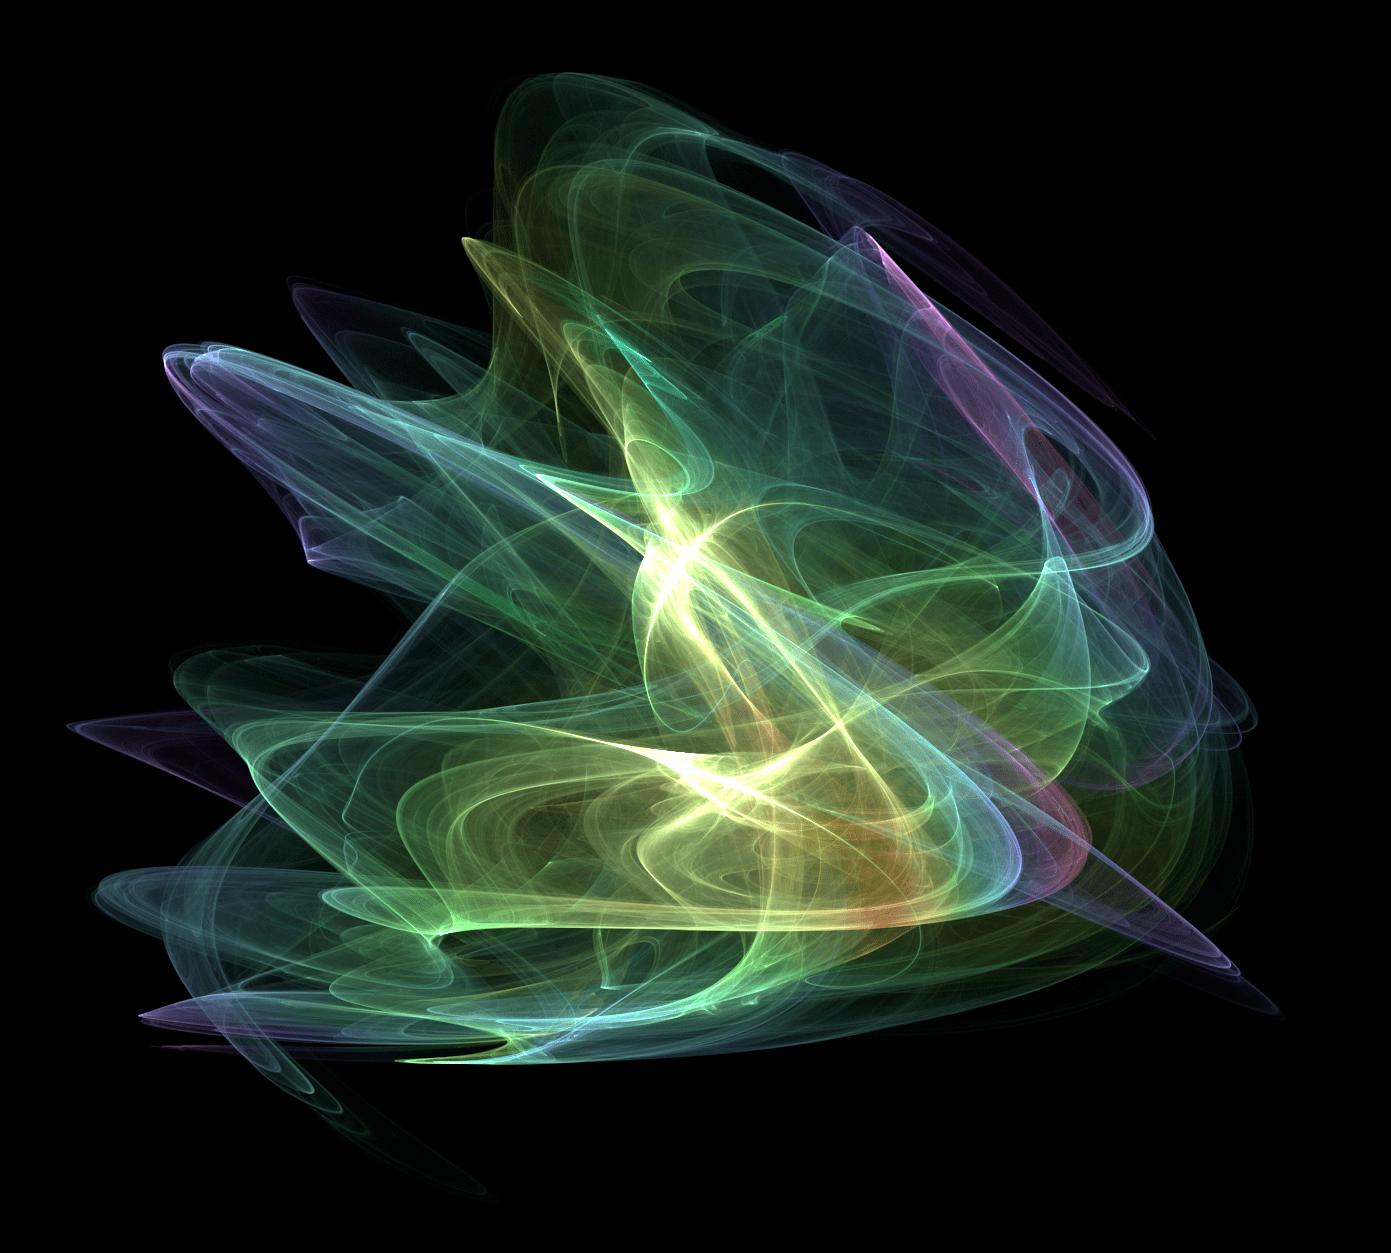
\includegraphics[height=3.2cm,width=3.7cm]{chaos/compressed/20_iter_alt.png}
		\caption{20 iterations}
	\end{subfigure}
	\begin{subfigure}[t]{0.24\textwidth}
		\centering
		\tiny
		
\includegraphics[height=3.2cm,width=3.7cm]{chaos/compressed/100_iter_altj.png}
		\caption{100 iterations}
	\end{subfigure}
	\begin{subfigure}[t]{0.24\textwidth}
		\centering
		\tiny
		
\includegraphics[height=3.2cm,width=3.7cm]{chaos/compressed/target_light.png}
		\caption{Ground truth}
	\end{subfigure}
	\caption{A series of trajectories for different parameters, demonstrating convergence to the true attractor.  The colormap is based on the speed and curvature of the trajectory, with rendering done using the program Chaoscope (available at {\href{http://www.chaoscope.org/}{http://www.chaoscope.org/}}). \label{fig:chaoscope}}
\end{figure}

Our first MMAP example considers the case of learning the dynamics parameters of a chaotic attractor.  
This constitutes a class Markovian state space model problem, specifically a Kalman smoother,
where we observe a noisy signal 
$y_t \in \real^{K}, \; t = 1,2,\dots,T$ in some $K$ dimensional observation space were each 
observation has a lower dimensional latent parameter $x_t \in \real^{D},  \; t = 1,2,\dots,T$.
In addition to an initial distribution $x_1 \sim \mathcal{N} \left(\mu_1, \sigma_1 I\right)$, our model is specified by 
\begin{subequations}
	\label{eq:Kalman}
\begin{align}
x_t = & A \left(x_{t-1}, \theta\right)+\delta_{t-1}, \; & \delta_{t-1} \sim \mathcal{N} \left(0, \sigma_q I\right) \\
y_t = & C x_{t}+\varepsilon_{t}, \; & \varepsilon_{t} \sim \mathcal{N} \left(0, \sigma_y I\right)
\end{align}
\end{subequations}
where $I$ is the identity matrix, $C$ is a known $K \times D$ matrix, and $\mu_1,\sigma_1, \sigma_q$ 
and $\sigma_y$ are all known scalars.  Our aim is to learn the dynamics parameters $\theta$ given
$y_{1:T}$, marginalizing over the latent variables $x_{1:T}$.  We use
a uniform prior on the parameters $\theta$, which means that the MMAP values for $\theta$
coincide with their (constrained) MML values.  A synthetic dataset was generated with $T=500$ and
$K=20$ (see \cite{rainforth2017boppArxiv}).
Inference on \qmarg was carried out using SMC with 500 particles.  
Convergence results are given in Figure~\ref{fig:chaos} showing that BOPP comfortably 
outperforms the PMMH variants, while Figure~\ref{fig:chaoscope} shows the simulated 
attractors generated from the dynamics parameters output by various iterations of a 
particular run of BOPP.


\subsubsection{Hidden Markov Model with Unknown Number of States}

% !TEX root =  ../main.tex

\begin{figure*}[t]
	\centering
	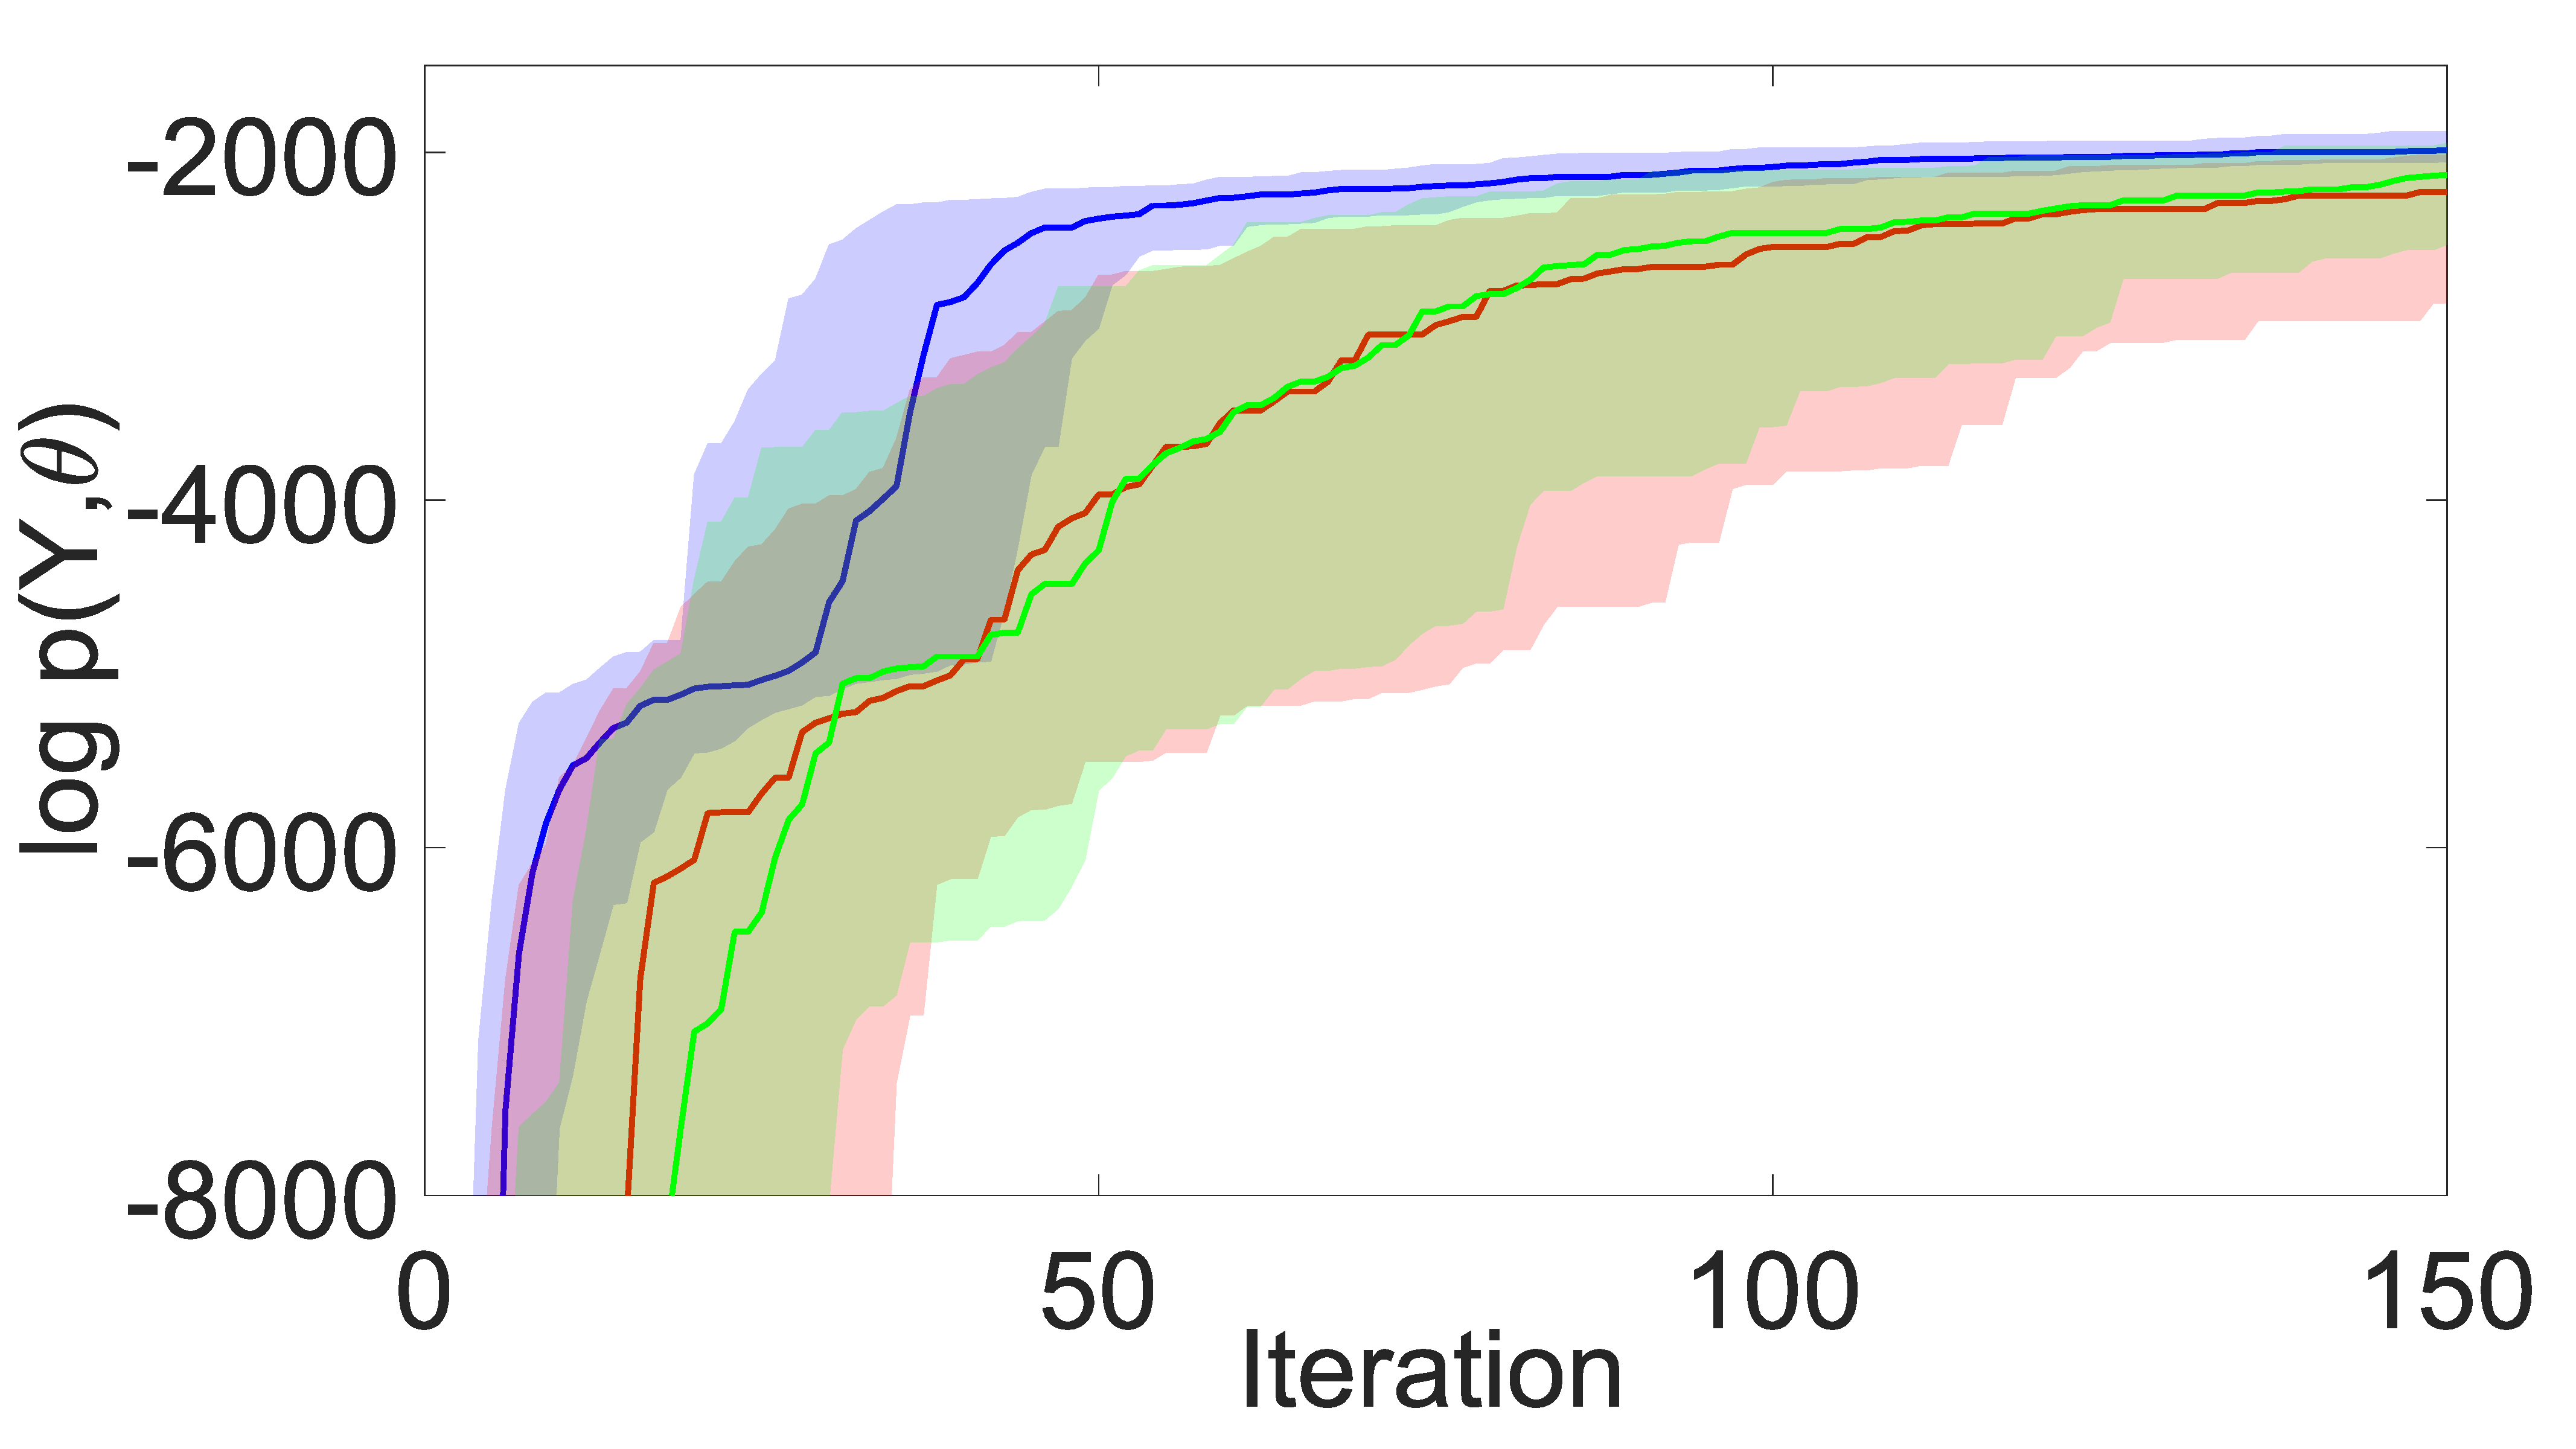
\includegraphics[width=2.72in]{hmm/hmm_ML}
	~~~~~~
	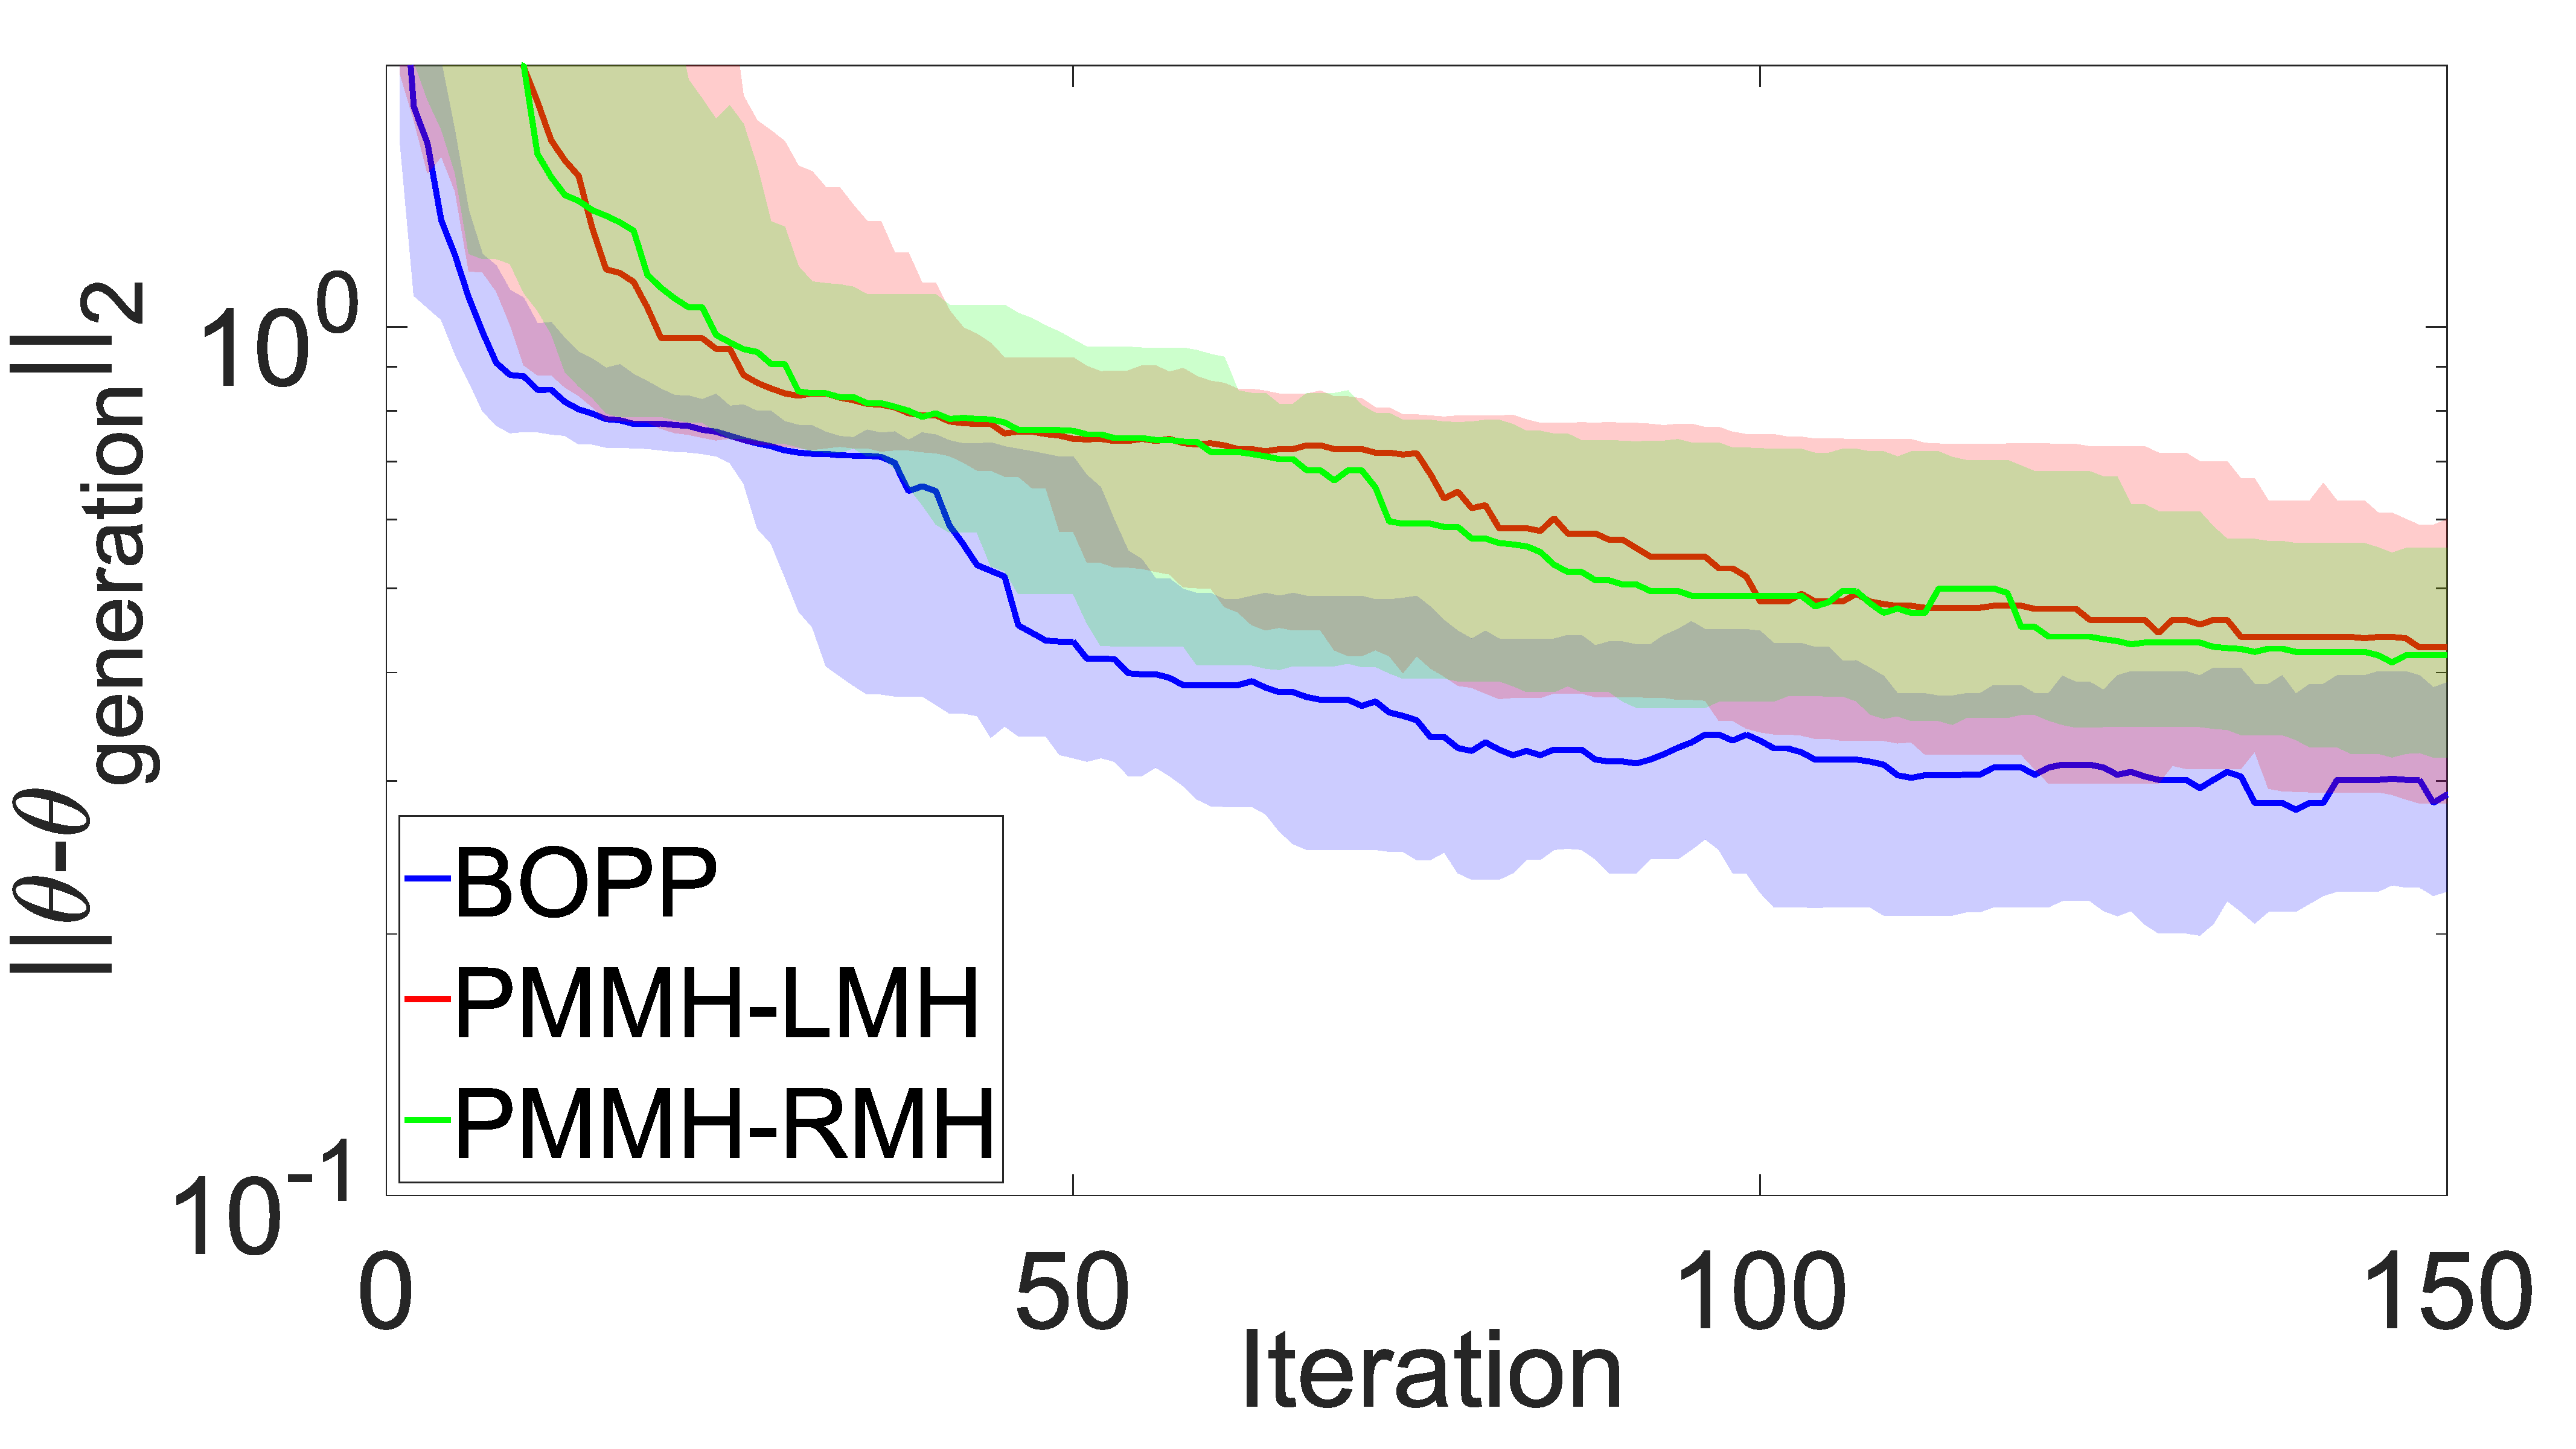
\includegraphics[width=2.72in]{hmm/hmm_distance}
	\caption{Convergence for HMM in terms of the cumulative best $\log p\left(Y,\theta\right)$ (\emph{left}) and distance to the ``true" $\theta$ used in generating the data (\emph{right}). Solid line shows median over 100 runs, whilst the shaded region the 25/75\% quantiles.  Note that for the distance to true $\theta$ was calculated by selecting the three states (out of the 5 generated) that were closest to the true parameters.  \label{fig:hmm}}
\end{figure*}

We finish by considering a hidden Markov model (HMM) with an unknown number of discrete possible states.  
This example demonstrates how BOPP can still be applied to models which conceptually have an 
unknown number of target variables, by generating all possible variables that might be needed, 
but then leaving some variables unused for some execution traces.  This avoids problems 
of varying reference measures so that the MMAP problem is well defined  and provides a 
function with a fixed number of inputs as required by the BO scheme.  From the BO 
perspective, the target function is simply constant for variations in an unused variable.

Our model places a uniform prior on the number of states $K \sim \textsc{Discrete}\{1,2,3,4,5\}$.
Each emission distribution corresponds to a Gaussian with unknown mean (which we wish to
optimize) and known variance.  
We marginalize over are the transition distribution parameters and the HMM latent states.  
Rather than constructing a model were the emission distribution
parameters only exist conditioned on the value of $K$, we generate variables for all $5$ emission
distributions that might be required, with only the first $K$ actually then used.  
A synthetic dataset was generated using $K=3$ and $T=1000$ observations.  Results of running BOPP are given
in Figure~\ref{fig:hmm}, again showing that BOPP outperforms these PMMH alternatives.  See~\cite{rainforth2017boppArxiv}
for further details.
